%!TEX root =presentation.tex
\begin{frame}
\frametitle{Riemann problem at junction}

For a junction $\jn$, let each link $\link \in Inc(\jn)\cup Out(\jn)$ have constant IC $\cvar_{\link}^0\in \mathbf{\cvar}_{\jn}$.

\begin{figure}
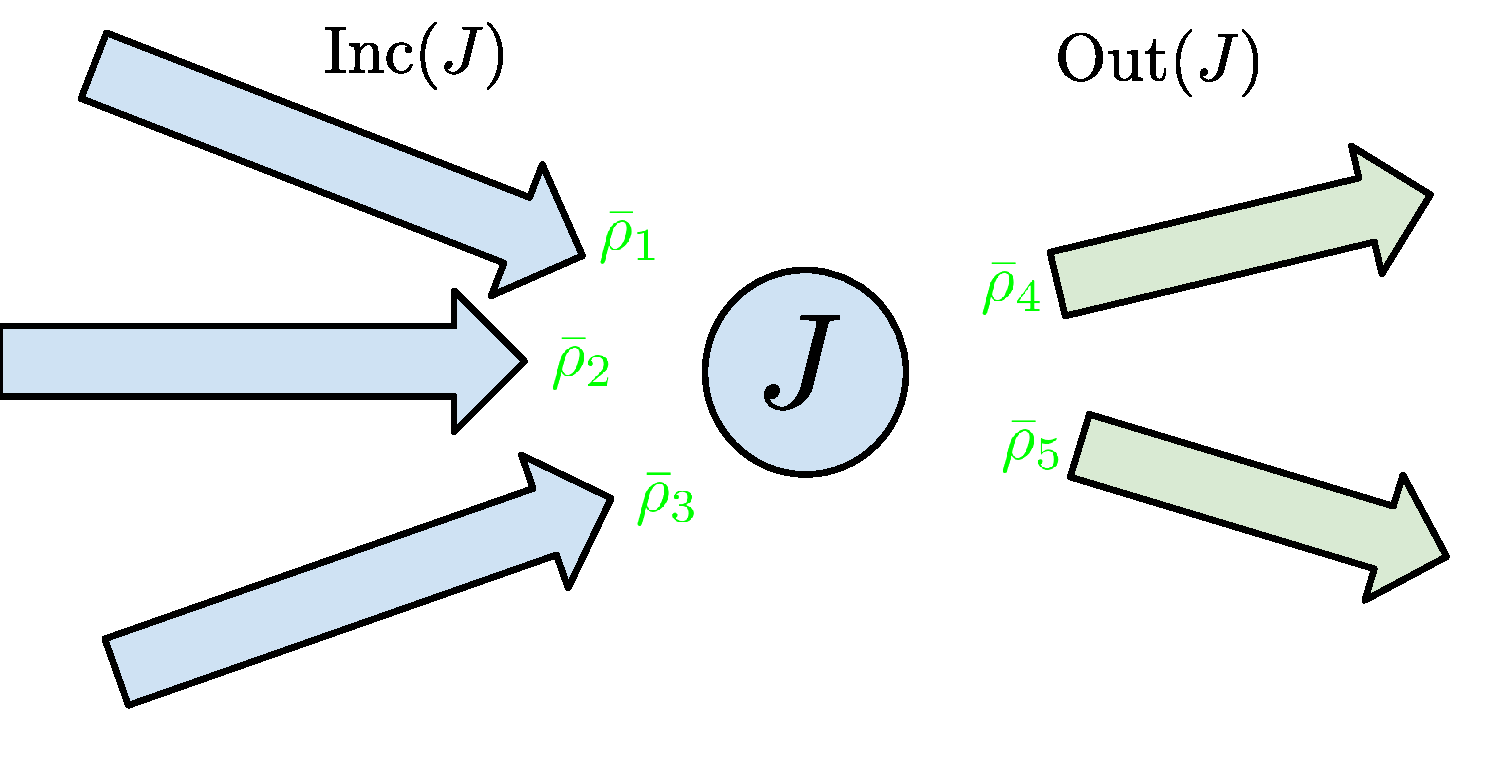
\includegraphics[width=.7\columnwidth]{figs-gen/junctions-riemann}
\end{figure}

\end{frame}

\begin{frame}

Define a \textbf{Riemann Solver} $\RS$:
\begin{eqnarray*}
\RS: & \mathbb{R}^{m+n} & \rightarrow\mathbb{R}^{m+n}\\
 & \tuple{\initstate_{1}}{\initstate_{\ninc+\nout}} & \mapsto\RS\tuple{\initstate_{1}}{\initstate_{\ninc+\nout}}=\tuple{\trace{\cvar}_{1}}{\trace{\cvar}_{\ninc+\nout}}
\end{eqnarray*}

where $\trace{\cvar}_{\link}$ provides the trace for link $\link$ for $t \ge 0$.

\begin{itemize}
    \item<2-3> Consider a specific link
\end{itemize}

\begin{figure}
\includegraphics<1>[width=.7\columnwidth]{figs-gen/junctions-riemann-rs}
\includegraphics<2>[width=.7\columnwidth]{figs-gen/junctions-riemann-rs-one}
\includegraphics<3>[width=.7\columnwidth]{figs-gen/riemann-junction}
\end{figure}

\end{frame}

\begin{frame}
\frametitle{Conditions on Riemann solver}

\begin{itemize}
    \item<1-> Self-similar
    \[
\RS\left(\RS\tuple{\initstate_{1}}{\initstate_{\ninc+\nout}}\right)=\RS\tuple{\initstate_{1}}{\initstate_{\ninc+\nout}}=\tuple{\trace{\cvar}_{1}}{\trace{\cvar}_{\ninc+\nout}}
\]
    \item<2-> All shockwaves must emanate outward from junction
    \begin{figure}
    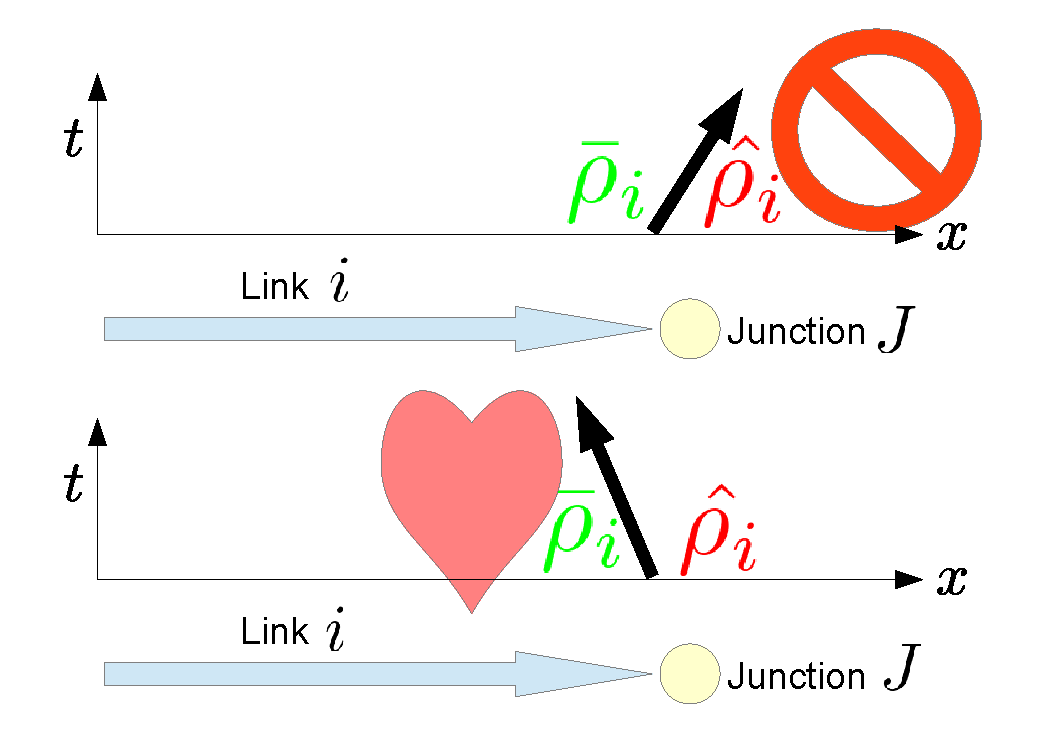
\includegraphics[width=.5\columnwidth]{figs-gen/shock}
    \end{figure}
    \item<3-> Conservation of mass
    \[
\sum_{i\in\Inc\left(\jn\right)}f\left(\trace{\cvar}_{\link}\right)=\sum_{j\in\Out\left(\jn\right)}f\left(\trace{\cvar}_{j}\right)
\]
\end{itemize}

\end{frame}


% \begin{frame}
% \frametitle{Riemann solver for linear flux function}
% \begin{example}
% On board...
% \end{example}
% \end{frame}
